\begin{figure}[htbp]
  \centering
  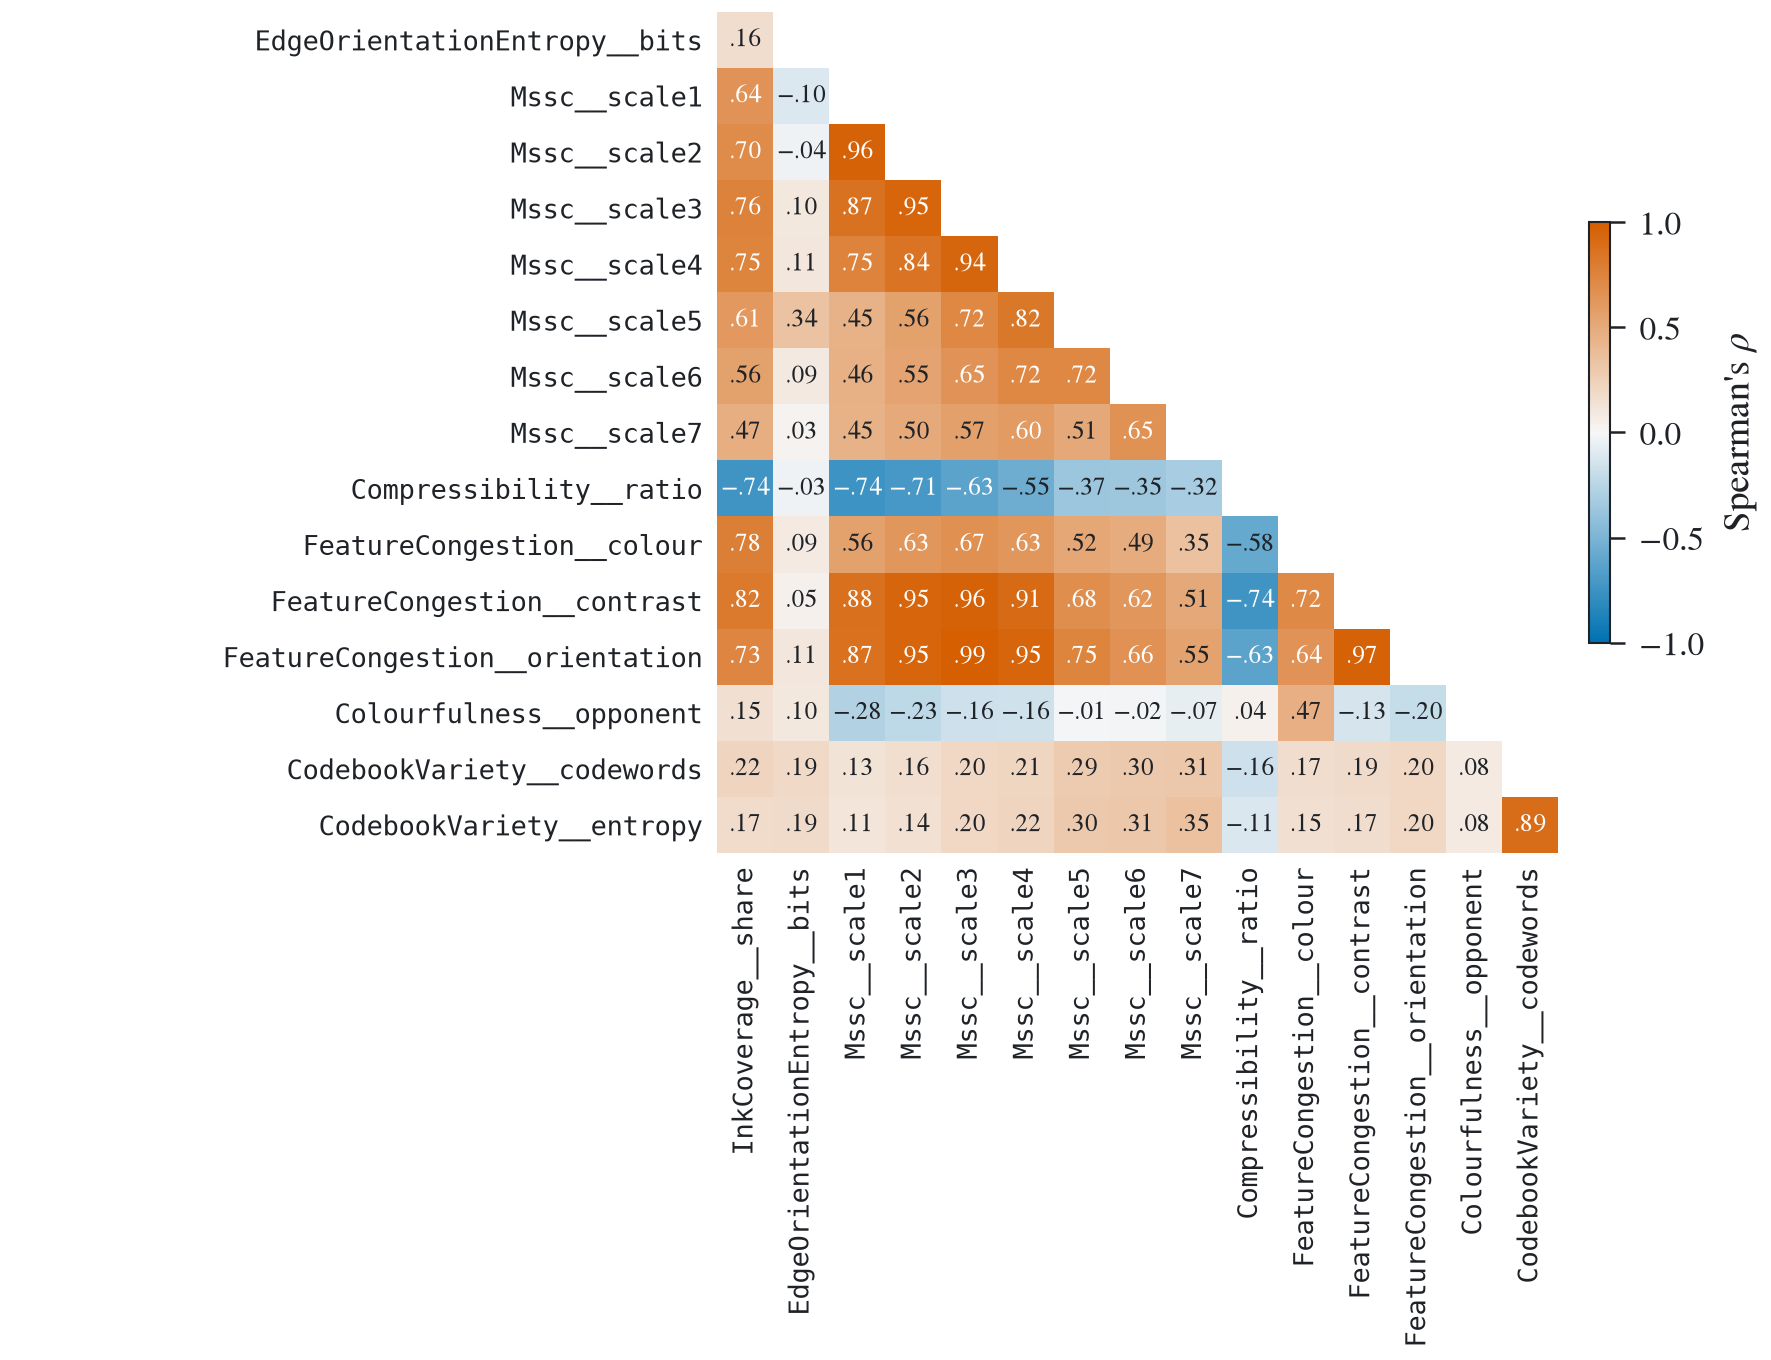
\includegraphics[width=15.00cm]{figures/generic_measure_correlations.png}
  \caption{Spearman's correlations among the 15 columns of the generic image measures and with ink coverage (\texttt{Trivial\_\_InkCoverage\_\_share}, first), over the 397 pages; blue where negative, vermillion where positive. Code names without their family's prefix (\texttt{Generic\_\_}).}
  \label{fig:generic_measure_correlations}
\end{figure}
